

\usetikzlibrary{positioning}  % Required for node placement like "below=0.5cm of..."
\usetikzlibrary{arrows.meta}  % Required for the sleek ">={stealth}" arrows
\usetikzlibrary{shapes}       % Good to have for advanced node shapes
\setcounter{chapter}{7}
\renewcommand{\thetheorem}{\thechapter.\arabic{theorem}}
\setcounter{theorem}{0}

\chapter{Span and Linear Combinations}

\subsection{Preparation}

Let $V$ be a vector space over a field $K$. Let $S \subseteq V$ be a subset (which is not necessarily a linear subspace). We aim to answer two fundamental and closely related questions:
\begin{enumerate}
    \item What is the \textit{smallest} linear subspace of $V$ that contains $S$?
    \item What structure do we obtain if we consider the subset of $V$ formed by taking all possible linear combinations of elements from $S$?
\end{enumerate}

To formalize the concept of a "smallest" subspace, we must first prove that the intersection of any collection of subspaces remains a subspace.

\begin{lemma}
Let $V$ be a vector space over $K$. Let $\{W_i\}_{i \in I}$ be a collection of linear subspaces $W_i \subseteq V$ of $V$, indexed by an arbitrary set $I$. Then their intersection
\[
W := \bigcap_{i \in I} W_i
\]
is a linear subspace of $V$.
\end{lemma}

\begin{proof}
First, since every $W_i$ is a subspace, the zero vector $0_V$ is contained in every $W_i$. Therefore, $0_V \in \bigcap_{i \in I} W_i = W$.

Next, let $a_1, a_2 \in K$ and $w_1, w_2 \in W$. We must show that $a_1 w_1 + a_2 w_2 \in W$. 
Choose an arbitrary index $j \in I$. Since $w_1, w_2 \in \bigcap_{i \in I} W_i$, we trivially have $w_1, w_2 \in W_j$. Because $W_j \subseteq V$ is itself a linear subspace, it is closed under addition and scalar multiplication, which implies:
\[
a_1 w_1 + a_2 w_2 \in W_j
\]
Since we have proved that $a_1 w_1 + a_2 w_2 \in W_j$ holds for every $j \in I$, we conclude that:
\[
a_1 w_1 + a_2 w_2 \in \bigcap_{i \in I} W_i = W
\]
This proves that $W$ is a linear subspace.
\end{proof}

\begin{definition}[Span]
Let $S \subseteq V$ be a subset. We define the \textit{span} of $S$ as the intersection of all linear subspaces of $V$ that contain $S$:
\[
\Sp(S) := \bigcap_{\substack{S \subseteq W \subseteq V \\ W \text{ is a subspace}}} W
\]
By convention, the span of the empty set is defined as the zero subspace: $\Sp(\emptyset) := \{0_V\}$.
\end{definition}

\begin{definition}[Linear Combination]
Let $\alpha_1, \dots, \alpha_n \in K$ be scalars and $w_1, \dots, w_n \in V$ be vectors. A \textit{linear combination} of the vectors $w_1, \dots, w_n$ with coefficients $\alpha_1, \dots, \alpha_n$ is the vector:
\[
\alpha_1 w_1 + \dots + \alpha_n w_n \in V \quad \left(\text{or equivalently, } \sum_{i=1}^n \alpha_i w_i\right)
\]
\end{definition}

\begin{importantremark}
In this course, we consider \textbf{only finitely many elements} in the sums of linear combinations. Infinite sums require topological notions of limits and convergence, which fall outside the scope of general vector spaces.
\end{importantremark}

\begin{lemma}
Let $\emptyset \ne S \subseteq V$. Then $\Sp(S)$ is exactly the set of all possible linear combinations of vectors from $S$:
\begin{align*}
\Sp(S) &= \{a_1 w_1 + \dots + a_n w_n \mid n \in \mathbb{N}, a_i \in K, w_i \in S\} \\
&= \text{subset of } V \text{ obtained by taking all possible linear combinations of vectors from } S.
\end{align*}
\end{lemma}

\begin{remark}
The set $S$ itself can be finite or infinite. Regardless of the size of $S$, each individual linear combination uses only a finite number of elements from $S$.
\end{remark}

\begin{proof}
Let us denote the set of all linear combinations by $\widetilde{\Sp}(S) = \{a_1 w_1 + \dots + a_n w_n \mid n \in \mathbb{N}, a_i \in K, w_i \in S\}$. 

Before diving into the algebra, let us visualize the logical strategy of the proof. We will establish three facts, which together force $\Sp(S) = \widetilde{\Sp}(S)$:

\begin{center}
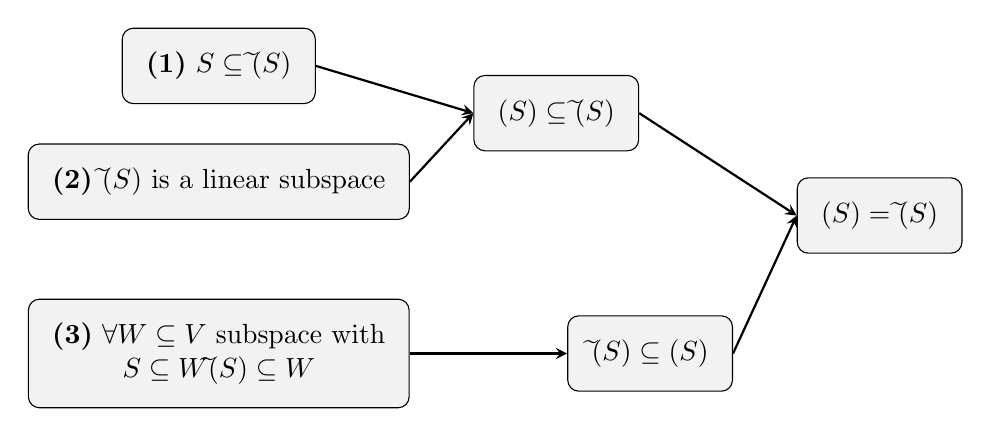
\begin{tikzpicture}[
    node distance=1.5cm and 2cm,
    box/.style={draw, rounded corners, fill=gray!10, align=center, inner sep=2ex},
    arrow/.style={->, thick, >=stealth}
]
    % Left Column (The 3 Facts)
    \node[box] (n1) {\textbf{(1)} $S \subseteq \widetilde{\Sp}(S)$};
    \node[box, below=0.5cm of n1] (n2) {\textbf{(2)} $\widetilde{\Sp}(S)$ is a linear subspace};
    \node[box, below=1cm of n2] (n3) {\textbf{(3)} $\forall W \subseteq V$ subspace with \\ $S \subseteq W \implies \widetilde{\Sp}(S) \subseteq W$};
    
    % Middle Column (Implications)
    \node[box, right=2cm of n1, yshift=-0.6cm] (p1) {$\Sp(S) \subseteq \widetilde{\Sp}(S)$};
    \node[box, right=2cm of n3] (p2) {$\widetilde{\Sp}(S) \subseteq \Sp(S)$};
    
    % Right Column (Conclusion)
    \node[box, right=2cm of p1, yshift=-1.3cm] (final) {$\Sp(S) = \widetilde{\Sp}(S)$};
    
    % Arrows mapping the logic
    \draw[arrow] (n1.east) -- (p1.west);
    \draw[arrow] (n2.east) -- (p1.west);
    \draw[arrow] (n3.east) -- (p2.west);
    
    \draw[arrow] (p1.east) -- (final.west);
    \draw[arrow] (p2.east) -- (final.west);
\end{tikzpicture}
\end{center}

Note that (1) and (2) imply that $\Sp(S) \subseteq \widetilde{\Sp}(S)$ because $\Sp(S)$ is defined as the intersection of \textit{all} subspaces containing $S$. Furthermore, (3) implies that $\widetilde{\Sp}(S) \subseteq \Sp(S)$ because $\Sp(S)$ is itself a valid subspace $W$ containing $S$.

\textbf{Proof of (1):} Let $v \in S$. Then we can write $v = 1 \cdot v \in \widetilde{\Sp}(S)$. Thus $S \subseteq \widetilde{\Sp}(S)$.

\textbf{Proof of (2):} 
First, $0_V \in \widetilde{\Sp}(S)$ because for any $w \in S$, $0 \cdot w = 0_V$. 
Second, let $u, v \in \widetilde{\Sp}(S)$. Then $u = a_1 w_1 + \dots + a_n w_n$ and $v = b_1 v_1 + \dots + b_m v_m$. Their sum:
\[
u + v = a_1 w_1 + \dots + a_n w_n + b_1 v_1 + \dots + b_m v_m \in \widetilde{\Sp}(S)
\]
Third, let $c \in K$ and $u \in \widetilde{\Sp}(S)$. Then:
\[
c \cdot u = c(a_1 w_1 + \dots + a_n w_n) = (c a_1)w_1 + \dots + (c a_n)w_n \in \widetilde{\Sp}(S)
\]
Thus $\widetilde{\Sp}(S)$ is closed under addition and scalar multiplication, making it a subspace.

\textbf{Proof of (3):} Let $W \subseteq V$ be an arbitrary subspace such that $S \subseteq W$. Let $u \in \widetilde{\Sp}(S)$. Then $u = a_1 w_1 + \dots + a_n w_n$ with elements $w_i \in S$. Since $S \subseteq W$, we know $w_i \in W$. Since $W$ is a subspace, it is closed under scalar multiplication and finite addition, which guarantees $a_1 w_1 + \dots + a_n w_n \in W$. So $u \in W$. Thus $\widetilde{\Sp}(S) \subseteq W$.
\end{proof}

\subsection{Checking for Span: The Bridge to Computations}

Up to this point, our definition of the span has been highly abstract. We know that if $S = \{w_1, \dots, w_n\}$ is a finite set, we can drop the set brackets and write its span as the set of all possible linear combinations:
\[
\Sp(w_1, \dots, w_n) = \{x_1 w_1 + \dots + x_n w_n \mid x_1, \dots, x_n \in K\}
\]
However, as a student of linear algebra, you should immediately ask a practical, computational question: \textbf{If I hand you a specific, concrete target vector $w$, how can we mathematically determine whether or not $w \in \Sp(w_1, \dots, w_n)$?}

To build our intuition, let us translate this abstract geometric question into algebra. Suppose our vector space is $V = K^m$. This means our vectors are just column vectors with $m$ entries. 

If $w$ is indeed in the span of $w_1, \dots, w_n$, there must exist some scalar "weights" $x_1, \dots, x_n \in K$ that allow us to build $w$. In other words, we need to solve the vector equation:
\begin{equation} \label{eq:vector_combo}
x_1 w_1 + x_2 w_2 + \dots + x_n w_n = w
\end{equation}

Let us write these vectors out explicitly by their components:
\[
w_1 = \begin{pmatrix} w_{1,1} \\ w_{2,1} \\ \vdots \\ w_{m,1} \end{pmatrix}, \quad w_2 = \begin{pmatrix} w_{1,2} \\ w_{2,2} \\ \vdots \\ w_{m,2} \end{pmatrix}, \quad \dots \quad , \quad w_n = \begin{pmatrix} w_{1,n} \\ w_{2,n} \\ \vdots \\ w_{m,n} \end{pmatrix}, \quad \text{and target } w = \begin{pmatrix} w_1 \\ w_2 \\ \vdots \\ w_m \end{pmatrix}
\]

If we substitute these columns into Equation \eqref{eq:vector_combo} and perform the scalar multiplication and vector addition component by component, we get a massive single column vector on the left side:
\[
\begin{pmatrix} 
x_1 w_{1,1} + x_2 w_{1,2} + \dots + x_n w_{1,n} \\ 
x_1 w_{2,1} + x_2 w_{2,2} + \dots + x_n w_{2,n} \\ 
\vdots \\ 
x_1 w_{m,1} + x_2 w_{m,2} + \dots + x_n w_{m,n} 
\end{pmatrix} 
= 
\begin{pmatrix} w_1 \\ w_2 \\ \vdots \\ w_m \end{pmatrix}
\]

Look closely at the left-hand side. This is exactly the definition of matrix-vector multiplication! We can seamlessly separate the known vector components from the unknown scalar weights $x_i$ by factoring this out into a coefficient matrix $A$ multiplied by a variable vector $x$:
\[
\underbrace{\begin{pmatrix} 
w_{1,1} & w_{1,2} & \dots & w_{1,n} \\ 
w_{2,1} & w_{2,2} & \dots & w_{2,n} \\ 
\vdots & \vdots & \ddots & \vdots \\ 
w_{m,1} & w_{m,2} & \dots & w_{m,n} 
\end{pmatrix}}_{\text{Matrix } A \text{ (whose columns are } w_i)}
\underbrace{\begin{pmatrix} x_1 \\ x_2 \\ \vdots \\ x_n \end{pmatrix}}_{\text{Vector } x}
= 
\underbrace{\begin{pmatrix} w_1 \\ w_2 \\ \vdots \\ w_m \end{pmatrix}}_{\text{Target } w}
\]

This reveals one of the most profound and useful insights in all of linear algebra: \textbf{A matrix-vector product $A \cdot x$ is simply a linear combination of the columns of $A$, weighted by the entries of $x$.} 

\begin{theorem}
Let $w, w_1, \dots, w_n \in K^m$. Let $A \in \M_{m \times n}(K)$ be the matrix whose columns are exactly the vectors $w_1, \dots, w_n$. Then the target vector $w$ is in the span of $w_1, \dots, w_n$ if and only if the system of linear equations $A \cdot x = w$ has at least one solution $x = (x_1, \dots, x_n)^T \in K^n$. 
\[
w \in \Sp(w_1, \dots, w_n) \iff \text{The system } A \cdot x = w \text{ is consistent.}
\]
\end{theorem}

\begin{remark}[How to check this in practice]
Because of this beautiful equivalence, whenever you are asked "Is $w$ in the span of these vectors?", you do not need to guess the coefficients. You simply construct the augmented matrix $(A \mid w)$ and perform Gaussian elimination. If the resulting system yields a contradiction, the vector is \textbf{not} in the span. If the system is solvable, the solutions $x_1, \dots, x_n$ are exactly the coefficients you need to build $w$.
\end{remark}

\subsection{Some spaces and how to generate them}

To conclude, let us look at some standard vector spaces and identify natural sets of "building block" vectors that span them entirely.

\begin{enumerate}
    \item \textbf{The Coordinate Space $K^n$:} 
    Let $e_1 = (1, 0, \dots, 0)$, $e_2 = (0, 1, 0, \dots, 0)$, $\dots$, $e_n = (0, \dots, 0, 1)$ be the standard basis vectors. Every vector $(x_1, \dots, x_n)$ can trivially be written as $x_1 e_1 + \dots + x_n e_n$.
    Then $K^n = \Sp(e_1, \dots, e_n)$. (\textbf{check!})
    
    \item \textbf{Bounded Polynomials $K[x]_d$:} 
    Let $W = K[x]_d$ be the space of polynomials over $K$ of degree $\le d$. 
    We can generate this space using the standard monomials:
    \[
    W = \Sp(1, x, x^2, \dots, x^d)
    \]
    
    \item \textbf{All Polynomials $K[x]$:} 
    Let $V = K[x]$ be the space of \textit{all} polynomials over $K$. 
    Generating this space requires an infinite set, as there is no maximum degree limit:
    \[
    V = \Sp(\{1, x, x^2, \dots, x^n, \dots\})
    \]
    
    \item \textbf{Spaces of Matrices $\M_{m \times n}(K)$:} 
    Consider the vector space of all $m \times n$ matrices over $K$. We can generate this entire space using the \textit{standard matrix basis}. 
    Let $E_{i,j}$ be the $m \times n$ matrix that has a $1$ in the $i$-th row and $j$-th column, and $0$ everywhere else. There are exactly $m \cdot n$ such matrices.
    
    For any arbitrary matrix $A = (A_{i,j}) \in \M_{m \times n}(K)$, we can pull it apart into a linear combination where the scalar weights are simply the matrix entries themselves:
    \[
    A = \sum_{i=1}^m \sum_{j=1}^n A_{i,j} \cdot E_{i,j}
    \]
    For instance, in $\M_{2 \times 2}(K)$, any matrix can be constructed like this:
    \[
    \begin{pmatrix} a & b \\ c & d \end{pmatrix} = a \begin{pmatrix} 1 & 0 \\ 0 & 0 \end{pmatrix} + b \begin{pmatrix} 0 & 1 \\ 0 & 0 \end{pmatrix} + c \begin{pmatrix} 0 & 0 \\ 1 & 0 \end{pmatrix} + d \begin{pmatrix} 0 & 0 \\ 0 & 1 \end{pmatrix}
    \]
    Thus, a matrix can be viewed as a "vector" built out of simpler matrices! We write:
    \[
    \M_{m \times n}(K) = \Sp(\{E_{i,j} \mid 1 \le i \le m, 1 \le j \le n\})
    \]
    (\textbf{check!!})
\end{enumerate}